\section{Realisation} \label{RefIntro}
Schon bei Projektstart wurde klar, dass es sich um sehr umfangreiche Anforderungen handelt. Es galt nicht nur eine Streaming Lösung zu implementieren, sondern es mussten auch alle Hardwarekomponenten getestet und angesteuert werden. Für die Bedienerseite musste eine funktionale Webseite einschließlich Webserver erstellt werden und ein Streaming-Server für die Konvertierung und Vernetzung der Sender und Empfänger musste konfiguriert werden. Viele \textbf{wichtige} bisher nicht genannte Anforderungen, z.B. Cybersicherheit, Authentifizierung wurden weitestgehend außer acht gelassen. Sie sind natürlich für eine endgültige industrielle Anwendung unerlässlich.\\

Das Projekt wurde in Teil-Aufgaben realisiert:
\begin{itemize}
\item Inbetriebnahme aller Hardwarekomponenten

\item Direktes Streamen von Audio und Video vom embedded System an PC
\item Aufsetzen eines Streaming-Servers im lokalen Netzwerk
\item Aufsetzen eines Webservers im lokalen Netzwerk, lokales hosting der Webseite
\item Direktes Streamen von Audio und Video vom embedded System an Streaming-Server
\item Anzeige des konvertierten Outputs des Streaming-Servers auf der Webseite
\item Streamen der PC Webcam an lokalen Streaming-Server
\item Zurück-Streamen vom Streaming-Server an embedded Hardware und Visualisierung
\item Hochladen der Webseite auf eine Online-Webspace
\item Aufsetzen eines Online-Streaming-Servers
\end{itemize}

\subsection{Inbetriebnahme der Hardware Komponenten}
Am Anfang des Projektes wurden alle Hardwarekomponenten bestellt und getestet. Raspberry PI B3+, Touchdisplays, Gehäuse, USB Lautsprecher, Webkameras mit Mikrofon und MMC Karten, siehe Lastenheft auf www.trello.com (Gruppe 15) für eine detaillierte Hardwareaufstellung. Danach kam die Installation des Betriebssystems RASPIAN auf den Raspberry PI3+ Boards und die Konfiguration eines Zugangs über SSH, siehe Kapitel \ref{RefRaspi}. Kleine Nebenarbeiten waren das softwareseitige Drehen des Displays und Touchdisplays, sowie das Upgraden und Updaten der vorinstallierten Pakete.\\
Für Audio und Video Tests wurden *.mp4 Files und *.wav Dateien abgespielt, siehe Kapitel \ref{RefLautsprecher}. WLAN befindet sich bereits bei PI3+ als Komponente auf dem Board und musste nur konfiguriert werden. Die Mikrofon Tests gestalteten sich anspruchsvoller und es wurden Facebook Chat und WebRTC Internet Beispiele verwendet.

\subsection{Streaming: embedded System > Server > Webseite}
Um A/V Streaming auf dem Raspberry zu starten, wurden ffmpeg und gstreamer mit den 
vorkompilierten Paketen über den Paketmanager installiert. Wobei gstreamer den vollen Funktionsumfang (verglichen mit Ubuntu 18) hatte. Für Installationsanleitung und kompletter Liste der Testbefehle zu gstreamer, siehe Kapitel \ref{RefGstreamer}. \\
Die Verwendung von ffmpeg gestaltete sich jedoch problematisch. Die Pakete des Paketmanagers unterstützten weder ffserver noch ffplay und es fehlten Abhängigkeiten zu diversen Bibliotheken. Es war nötig ffmpeg aus den Quellen zu bauen, siehe Kapitel \ref{RefFFmpeg} mit Schritt für Schritt Anleitung und alle durchgeführten Tests. Bei der Installation stellte sich heraus, dass ffserver nicht mehr in der aktuellen Version 4 unterstützt wird und es wurde via Git die Version 3.4 ausgecheckt. Dies bewirkte eine Kettenabhängigkeit der x264 Bibliothek, deren Version nun ebenfalls herunter gesetzt werden musste. Schließlich stand eine voll funktionsfähige ffmpeg, ffserver und ffplay Version bereit.\\ 

\textbf{Direktes A/V Streamen vom embedded System > PC}\\
Versuche mit ffmpeg A/V Streaming wiesen ein Delay von >2.5s zwischen senden und empfangen auf. Die Testergebnisse sind in Tabelle \ref{tbl:beispieltabelle} Kapitel \ref{RefVergleich} zusammengefasst. Der Stream wurde mit ffmpeg erzeugt und an den ffserver auf dem PC geschickt. Das Ergebnis \textbf{(m)} in Tabelle \ref{tbl:beispieltabelle} stellte das KO Kriterium dar. 2.5 Sekunden waren zuviel, um einen interaktiven Chat zu gestalten. PC seitig konnte daran nichts geändert werden. ffplay, mplayer und vlc wurden ohne Verbesserung des Ergebnisses getestet.\\
Gstreamer konnte dieses Ergebnis bei weitem übertreffen. A/V Streaming ohne Server war nahezu ohne Verzögerung ca. 0.1s, siehe Testergebnis \textbf{(h)} in Tabelle \ref{tbl:beispieltabelle}, Kapitel \ref{RefVergleich}. Gstreamer erfüllte damit die Anforderung und wurde im weiteren Projekt verwendet, um A/V direkt an den Streaming-Server zu senden.\\

\textbf{Aufsetzen eines Streaming-Servers im lokalen Netzwerk}\\
Die Auswahl eines OpenSoure Streaming Servers gestaltete sich schwierig. Die Anforderung einen A/V Stream möglichst Overhead frei, z.B. RTP/UDP Format, in ein Web natives Format zu konvertieren erforderte viel Recherchezeit. Dazu kommt noch, dass veröffentlichte Projekte meistens nicht passend sind und z.B. auf Browser zu Browser Streaming basieren. Alternativ handelt es sich um Streaming-Lösungen, die ganz ohne Browser arbeiten. Die gesetzte Anforderung aus einem eigenen Programm ohne Browser auf eine Webseite zu streamen und wieder zurück, erschwerte den Fortschritt des Projektes. Dazu kam noch, dass zwar Video Streaming generell gut dokumentiert ist, aber in Kombination mit Audio nicht häufig Verwendung findet. Das liegt hauptsächlich daran, dass die meist verkaufte RASPI-CAM kein Mikrofon besitzt und deshalb fast alle Tutorials und Dokumentationen nur Video Streaming beschreiben. Viele Start-Ups werben mit Lösungen, welche die A/V Anforderung im Projekt erfüllen würden. Es scheint ein Bereich unter aktiver Entwicklung zu sein, wie von und zu embedded Systemen A/V gestreamt werden kann.\\
Schließlich wurden UV4L und das Janus-Gateway in die engere Auswahl gezogen. Die UV4L Bibliothek erwähnt zwar eine Einsatzmöglichkeit auch ohne Webbrowser auf den Klientseite. Es konnte jedoch keine ausreichende Dokumentation gefunden werden, wie UV4L zum direkten A/V Streaming verwendet wird. Beim Janus-Gateway stand zumindest eine Standard-Konfiguration für RTP zu WebRTC bereit und in Foren werden Probleme nicht korrekter Konfiguration diskutiert. Auch ist das Empfangen von gstreamer RTP-Paketen möglich. Die Installation und Konfiguration des Janus-Gateways ist in Kapitel \ref{RefJanus} beschrieben. Das Janus-Gateway wurde im weiteren Projektverlauf verwendet, um mehrere RTP Streams von embedded Systemen zu empfangen und als WebRTC Streams via http auf eine Webseite weiterzuleiten.\\

\textbf{Aufsetzen eines Webservers im lokalen Netzwerk, Hosting der Webseite}\\
Als Webserver wurde nginx ausgewählt, um eine Webseite im lokalen Netzwerk zu hosten. Die Demo-Webseiten des Streaming-Servers benötigen noch diverse Anpassungen, um z.B. den Admin/Monitor verwenden zu können. Erst danach steht mit nginx eine vollwertige Entwicklungsumgebung zur Verfügung. Installation und Konfiguration von nginx wird in Kapitel \ref{Refnginx} erklärt.\\

\textbf{Direktes Streaming von Audio und Video vom embedded System an den Streaming-Server}\\
Gstreamer Befehle für die Übertragung von A/V vom Raspberry an das Janus-Gateway sind in Kapitel \ref{RefGstrToJanus} aufgelistet.

\subsection{Webseite zur Anzeige der Videostreams}
Die Janus-Installation enthält bereits Demowebseiten für die Anzeige der WebRTC Streams und Werkzeuge für die Konfiguration von Chaträumen. Mittels einer Debug Admin/Monitor Seite können eingehende Streams, Anzahl der Pakete, IP-Adressen usw. angezeigt werden. Der bereit gestellte Javascript-Code kann verwendet werden, um interaktiv Kamera und Mikrofon des Bedieners auszuwählen. Im Rahmen des Projektes wurde durch Änderung der Demowebseiten eine funktionale Testwebpage gestaltet, um wahlweise die A/V Streams verschiedener emb.Systeme anzeigen zu können.\\

\begin{minipage}{\textwidth}
    \begin{center}
        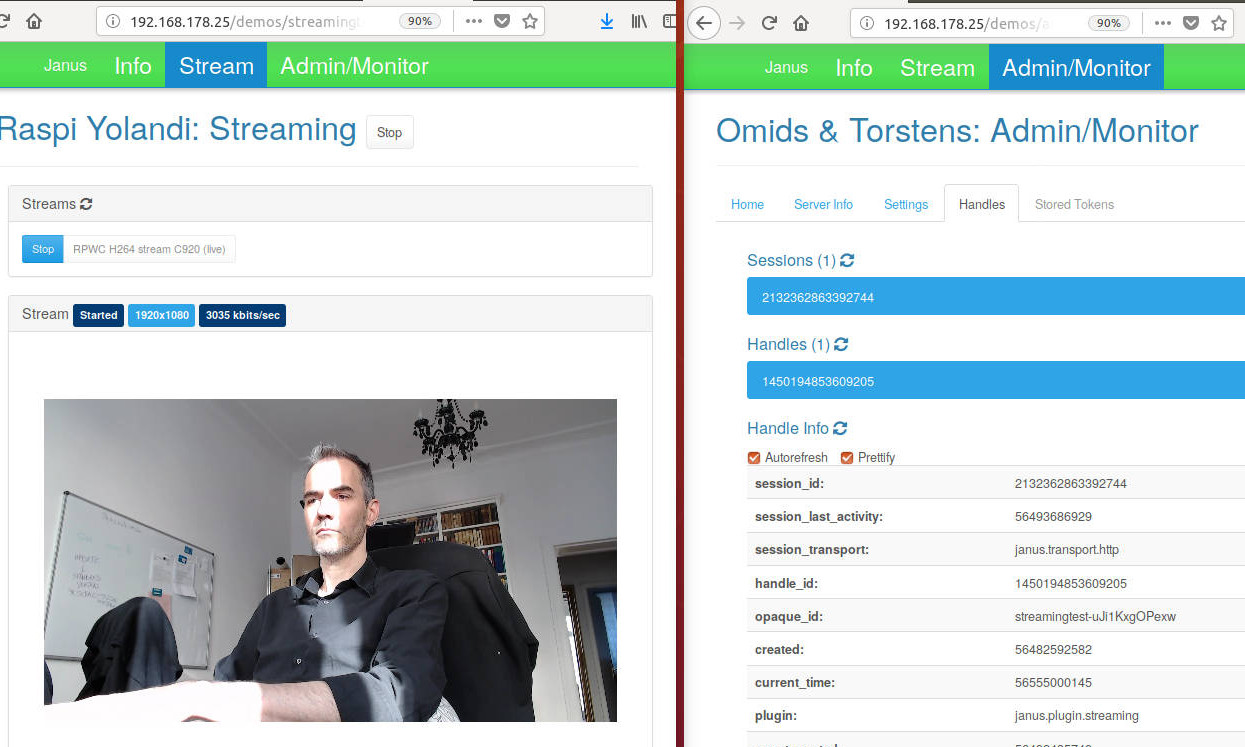
\includegraphics[scale=0.27]{img/janusweb.jpg} 
    \end{center}
\end{minipage}
\begin{center}
Adaptierte Website zur Anzeige der A/V WebRTC-Streams
\end{center}

\subsection{Streaming: PC > Server > Anzeige auf embedded System}
Wie der Test \textbf{(i)} in Tabelle \ref{tbl:beispieltabelle} Kapitel \ref{RefVergleich} gezeigt hat, ist gstreamer ungeeignet, um A/V auf den Raspberry zurück zu streamen. Die Framerate konnte nicht festgestellt werden, da das Entpacken und Decodieren der Formate zu langsam ist. Die CPU Leistung ist nicht ausreichend. Es wurden VP8, h264 Komprimierung und auch raw getestet, jedoch ohne Erfolg.\\

Ffmpeg blieb mit dem Testergebnis \textbf{(n)} mit >1.5s Delay die einzige funktionale Lösung. Der ffserver wurde so konfiguriert, dass die eingehenden http Pakete zu webm konvertiert werden. Auf dem Raspberry werden diese nur noch zur Anzeige gebracht, ohne aufwändiges Dekodieren. In Kapitel \ref{RefBack} sind die Konfiguration und Kommandozeilen-Eingaben aufgelistet. Das WebM Format kann auch im Browser angezeigt werden. Auf dem Raspberry trat jedoch im Browser ein Delay von15s auf! Alle Versuche A/V auf den Raspberry zurück zustreamen resultierten in 100\% CPU Last. Die Bibliotheken verwenden zwar Hardwareunterstüzung beim Kodieren und Komprimieren der Videoframes, aber nicht beim Dekodieren. Es müsste noch untersucht werden, ob eine Hardwareunterstützung für beide Aufgaben gleichzeitig erfolgen kann und ob dies von den Bibliotheken unterstützt wird. Der Standard ist es, Video vom leistungsschwachen System mit Hardwareunterstützung zu verschicken.\\

\begin{minipage}{\textwidth}
    \begin{center}
        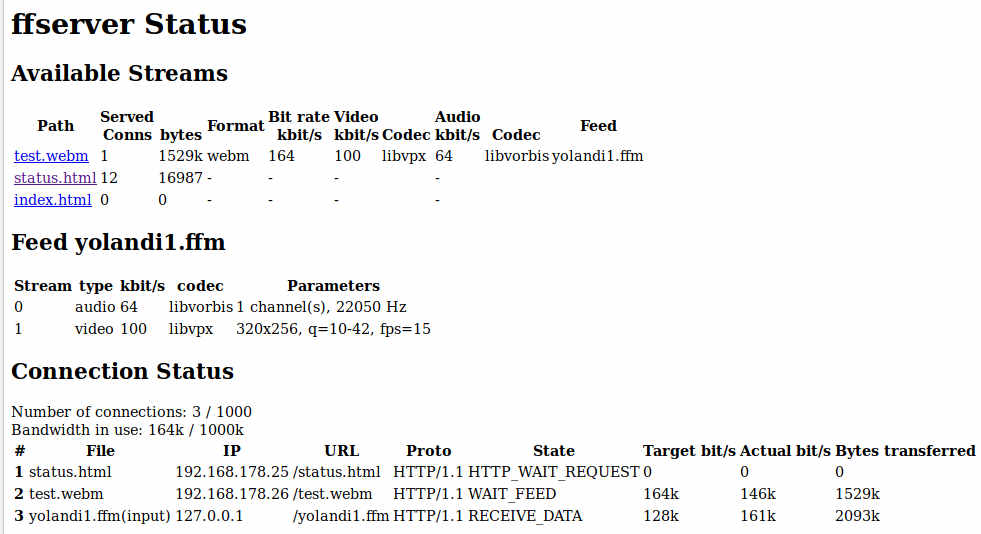
\includegraphics[scale=0.5]{img/statusff.jpg} 
    \end{center}
\end{minipage}
\begin{center}
Status ffserver Webpage zur Anzeige der verbundenen Streams
\end{center}

Der ffserver kann eine Status Webseite generieren, mit der fps, verbundene Klienten und eingehende Streams angezeigt werden können, siehe Screenshot.\\
Das zurück Streamen wurde für das Projekt mit ffmpeg auf PC Seite und ffserver auf dem Server realisiert. Der Raspberry Klient kann den webm http Stream direkt von der IP-Adresse und Port des Servers erhalten und via ffplay anzeigen. Als optionale Lösung könnte auch Audio getrennt von Video gesendet werden. Dann sollte Audio nahezu ohne Delay wiedergegeben werden können und Video mit ca. 1.5s Verzögerung.

\subsection{Online Setup}
Alle beschriebenen Tests und Installationen wurden auf PC und im lokalen Home-Netzwerk durchgeführt. Dies geschah mit dem Ausblick eine Lösung für das www zu entwickeln. Schließlich wurden gegen Ende es Projektes noch einige Tests im Internet durchgeführt. Dabei ging es um die Funktionalität der Webseite und die Ports des Streaming-Servers, leider konnten die Versuche noch nicht abgeschlossen werden.\\ 

\textbf{Hochladen der Webseite auf eine Online-Wespace}\\
Die angepasste Demo-Webseite wurde via Filezilla auf eine Strato-Webspace hochgeladen. Sie ist voll funktionsfähig und kann under \textit{www.witchplease.de} angezeigt werden. Der Janus-Webserver ist nicht durchgehend aktiv und wird nur zu Testzwecken gestartet. Wie schon am Anfang von Kapitel \ref{RefIntro} beschrieben wurde die Kommunikation noch \textbf{nicht} sicher gestaltet.\\

\textbf{Aufsetzen eines Online-Streaming-Servers}\\
Der Zugang zum Server erfolgte mit ssh und darauf aufbauend kann per VNC eine remote Desktopverbindung geöffnet werden. Eine Beschreibung ist in Kapitel \ref{RefStrato} zu finden. \\

\textbf{Webserver Verbindungstest}\\
Bei den gstreamer Versuchen wurde zuerst mit Wireshark untersucht, ob die RTP Pakete an den Ports der Servers ankommen. Der Screenshot zeigt den gstreamer Befehl und einen Ausschnitt der Wireshark gui.\\
Im oberen Bereich ist der gstreamer Befehl mit dem Audio udpsink host...5000 und Video udpsink...5001. Wireshark detektiert ankommende Pakete im Webserver (ip 85.214.211.169) vom raspberry pi (ip 77.14.37.230) an den UDP Ports 5000 (Audio Paketgröße 451) und UDP 5001 (Video Paketgröße 894).\\

\begin{minipage}{\textwidth}
    \begin{center}
        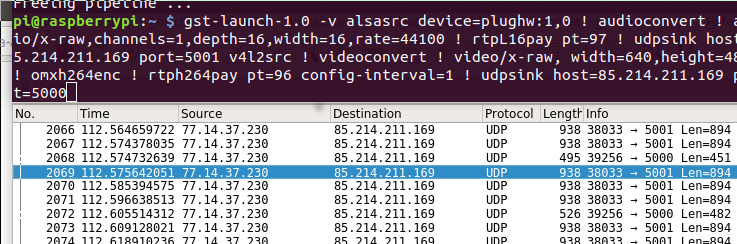
\includegraphics[scale=0.7]{img/wireshark.png} 
    \end{center}
\end{minipage}

\begin{center}
Wireshark detektiert ankommende Pakete an den Server-Ports
\end{center}

\subsection{Ergebnis}
Es konnte eine Streaming Lösung entwickelt werden, die A/V von mehreren Raspberry PiB3+ über WLAN auf eine Webseite streamt. Auf der Webseite kann ausgewählt werden, welcher Stream angezeigt werden soll. In einem Admin/Monitor können die verbundenen Streams mit umfangreichen Kenndaten ausgewertet werden. Im Detail sieht die Streaming Lösung wie folgt aus:
\begin{verbatim}
n * Raspi Webcam & Audio > gstreamer > RTP/UDP > Janus-Gateway > Http/WebRTC > Webseite
\end{verbatim}

Für das zurück Streamen, der am PC integrierten oder einer externen Webcam mit Audio, wurde ffmpeg und ffserver sowie ffplay verwendet. Dabei wird ein, mittels ffmpeg erzeugter Stream vom ffserver in das webm Format konvertiert und auf dem Raspberry mit ffplay ohne aufwändiges Dekodieren angezeigt. Im Detail sieht die zurück Streaming Lösung wie folgt aus:
\begin{verbatim}
PC Webcam & Audio > ffmepg > http > ffserver > http/webm > n * Raspi ffplay
\end{verbatim}

Die gesetzten Anforderungen konnten damit voll erfüllt werden. Es ist möglich von mehreren Raspberries auf eine Webseite zu streamen und die Webcam des Users auf alle verbundenen Raspberries zurück zu streamen. Auf dem Raspberry PI können alle Streams generiert und empfangen werden, ohne dass ein Webbrowser benötigt wird und verwendeten Bibliotheken ffmpeg und gstreamer können sogar auch direkt in eigene Programme integriert werden. Die Kommandozeilen-Befehle können z.B. auch direkt beim Systemstart aktiviert werden, so dass ein manuelles Aktivieren entfällt. Für den Bediener wurde eine einfach zu handhabende Webseite bereit gestellt, um die Streams anzuzeigen. \\
Zu allen verwendeten Werkzeugen wurden ausführliche Installationsanleitungen geschrieben und die Tests dokumentiert.\\

\textbf{Ausblick}\\
Ideal wäre das zurück Streamen auch über WebRTC zu realisieren. Die Javascript Bibliotheken sind verfügbar und ermöglichen dem User das Auswählen der gewünschten Kamera und des Mikrofons auf dem eigenen PC. UV4L könnte den Empfang des WebRTC Streams auf dem Raspberry PI ohne Browser realisieren.
